It is claimed in this section that you cannot make a Venn diagram for four sets using overlapping circles.
\begin{enumerate}[label=(\alph*)]
    \item What's swrong with the following diagram? (Hint: Where's the set $(A \cap D) \mybackslash (B \cup C)$?) \\
    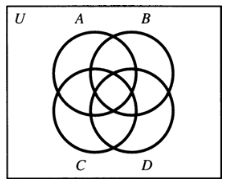
\includegraphics[width=5cm]{./4-Figure.png} \\    
    \item Can you make a Venn diagram for four sets using shapes other than circles?
\end{enumerate}

\textbf{Solution:}
\begin{enumerate}[label=(\alph*)]
    \item Fun fact, the number of sections in a Venn diagram of $n$ sets corresponds to the number of rows of a truth table of $n$ sets, that is to say, there is always $2^n$. Below is the case for $n = 3$. \\

    \
    
    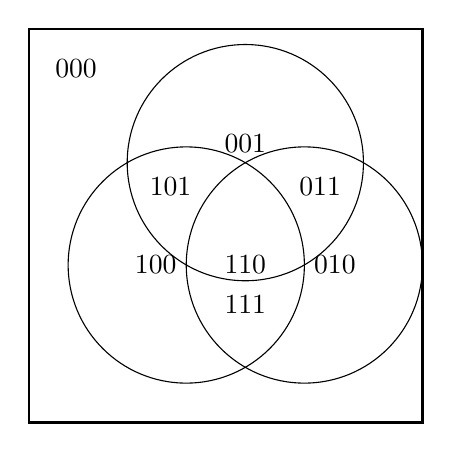
\begin{tikzpicture}
        % Define circles for A, B, and C
        \def\circleA{(0,0) circle (1.5cm)}
        \def\circleB{(1.5,0) circle (1.5cm)}
        \def\circleC{(0.75,1.3) circle (1.5cm)}
    
        % Fill the circles with white (default background)
        \begin{scope}
            \clip \circleA;
            \clip \circleB;
            \clip \circleC;
            \fill[white] \circleC;
        \end{scope}
    
        % Draw circles with labels and binary code for each section
        \draw \circleA node [text=black, left] {100};
        \draw \circleB node [text=black, right] {010};
        \draw \circleC node [text=black, above] {001};
        
        % Adding labels for overlapping sections
        \node at (0.75,0) {110};
        \node at (0.75,-0.5) {111};
        \node at (-0.2,1.0) {101};
        \node at (1.7,1.0) {011};
    
        % Label for the area outside all circles
        \node at (-1.4,2.5) {000};
    
        % Draw a square container around the Venn diagram
        \draw [thick] (-2, -2) rectangle (3, 3);
    \end{tikzpicture}

    If you count the number of regions in $(A \cap D) \mybackslash (B \cup C)$, you will count 14 sections, when there should be $2^4 = 16$. Also, in the given diagram $(A \cap D) \subseteq (B \cup C)$, so $(A \cap D) \mybackslash (B \cup C)$ does not exist, but in the corresponding truth table there is a row where elements belong to only $A$ and $D$, but not the others. Visually, that row should be present in the diagram, but it is not.
    \pagebreak
    \item It is beyond our interest as to why precisely circles are unable to illustrate a Venn diagram of 4 sets. Know that it can be done by replacing circles with ellipses, and note that we do in fact have 16 sections, the 15 non-empty pieces, and the container of the diagram.\\
    \fbox{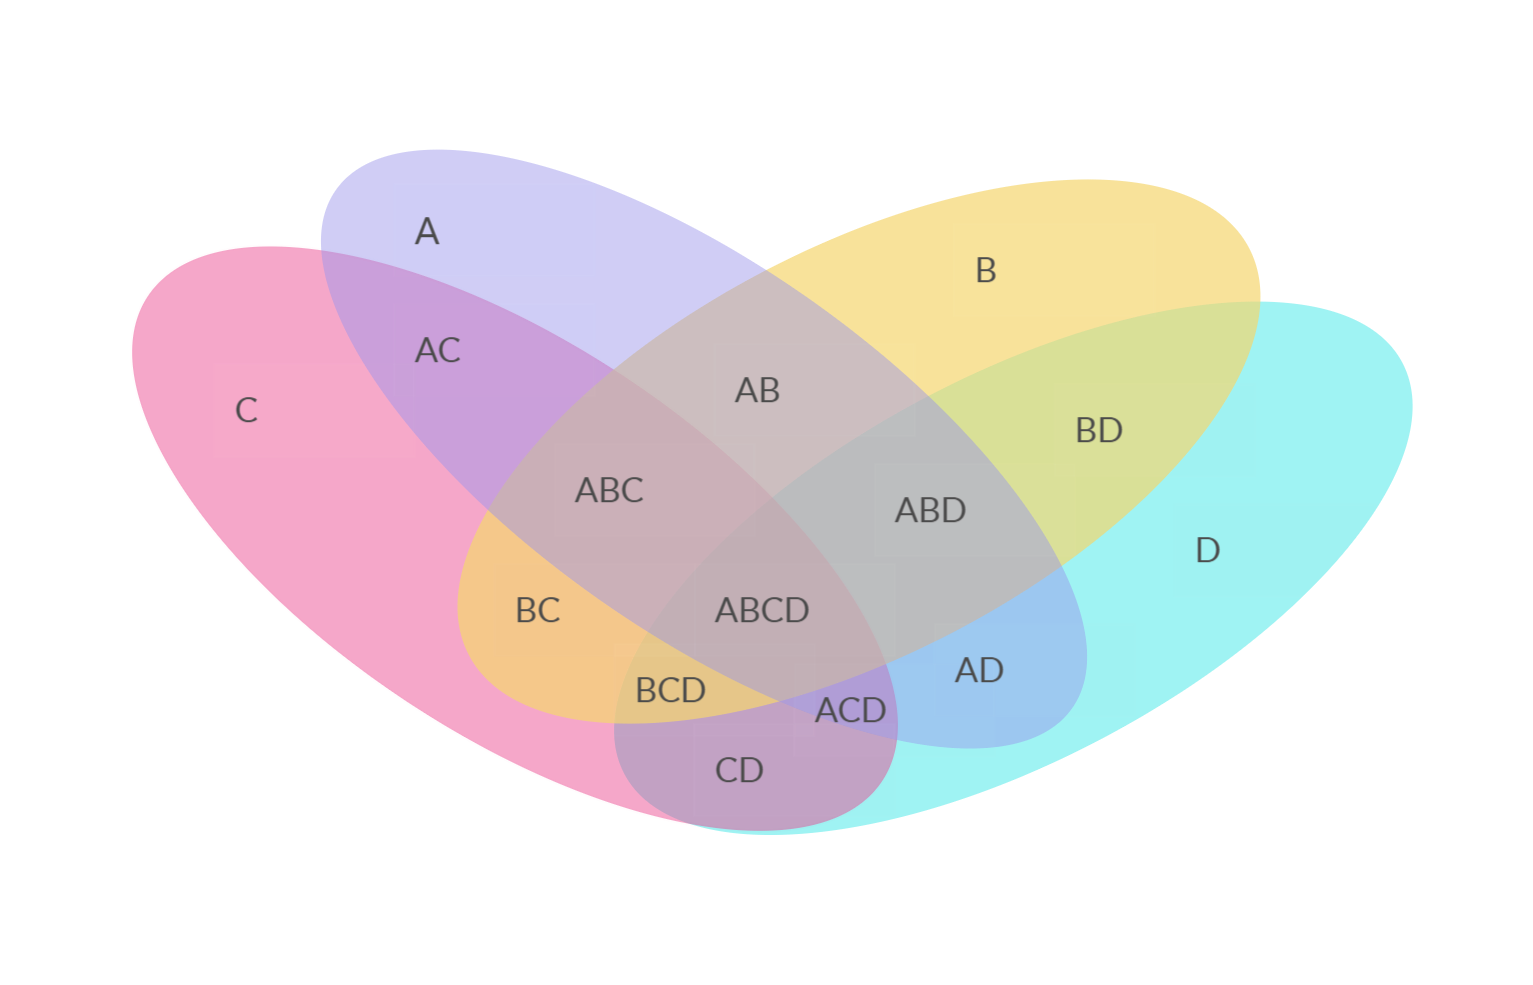
\includegraphics[width=15cm]{./4-Figure2.png}}
\end{enumerate}
\pagebreak